\documentclass{article}
\usepackage[utf8]{inputenc}
\usepackage{amsmath}
\usepackage{amssymb}
\usepackage{color}
\usepackage{enumitem}
\usepackage{fancyhdr}
\usepackage[margin=1in,top=1in,headheight=18pt]{geometry}
\usepackage{listings}
\usepackage{graphicx}
\usepackage{hyperref}
\usepackage{dirtree}
\usepackage{tikzsymbols}
\usepackage{wrapfig}
\usepackage{subfig}
\usepackage{tikz}
\usepackage{soul}
\usepackage[toc,page]{appendix}
\usepackage[style=authoryear-icomp,maxbibnames=9,maxcitenames=2,backend=biber]{biblatex}
\addbibresource{./Authors.bib}
% \bibliographystyle{plainnat}
\graphicspath{ {./images/} }

\hypersetup{
    colorlinks=true,
    linkcolor=blue,
    filecolor=magenta,      
    urlcolor=cyan,
    pdftitle={Overleaf Example},
    pdfpagemode=FullScreen,
    }
    
\newcommand{\ExternalLink}{%
    \tikz[x=1.2ex, y=1.2ex, baseline=-0.05ex]{% 
        \begin{scope}[x=1ex, y=1ex]
            \clip (-0.1,-0.1) 
                --++ (-0, 1.2) 
                --++ (0.6, 0) 
                --++ (0, -0.6) 
                --++ (0.6, 0) 
                --++ (0, -1);
            \path[draw, 
                line width = 0.5, 
                rounded corners=0.5] 
                (0,0) rectangle (1,1);
        \end{scope}
        \path[draw, line width = 0.5] (0.5, 0.5) 
            -- (1, 1);
        \path[draw, line width = 0.5] (0.6, 1) 
            -- (1, 1) -- (1, 0.6);
        }
    }


\definecolor{ao}{rgb}{0.0, 0.0, 1.0}
\hypersetup{
    colorlinks=false,
}

\urlstyle{same}

\setlength{\parindent}{0pt}

\newcommand{\ttt}[1]{\texttt{#1}}

\title{Assignment 2 Part 2 - Face Verification}
\author{Introduction to Deep Learning \\ Emeritus \& Carnegie Mellon University}
\date{} \\
\vspace{.1in}

\begin{document}
\pagenumbering{arabic}

\maketitle

\section{Overview}
Have you ever wondered how facial recognition works? In this assignment, we'll be tackling another real-world application of DL: face verification.\\

\textbf{Objective}: Given two pictures of human faces, determine if the faces belong to the same person.\\

\textbf{As with the last assignment, make sure you start this assignment early.} This pipeline will be a little complex, in order to give you exposure to what real DL work is like, and introduce you to some key concepts like transfer learning and embeddings. 

% \newpage
% % --------------------------------------

\subsection{Pipeline Overview}

We're going to take an indirect approach to this problem, using transfer-learning. You could take a more direct approach, but pipelines for that tend to be much more complicated to both implement AND train. Even though this approach is indirect, it's still valid, and indirect approaches with transfer learning are very common in DL.

\begin{enumerate}
    \item Classification
    \begin{itemize}
        \item Train a computer vision (CV) model to classify which person an image of a face belongs to
        \item The model will be a variation of \textbf{ResNet}, a landmark CV model that's still used today for benchmarking and DL theory.
            \begin{itemize}
                \item It's important you're familiar with this model, as it introduces important tricks that enable training of very deep models, and because it appears a lot in research.
            \end{itemize}
    \end{itemize}    
    \item Verification
    \begin{itemize}
        \item We can use the model we trained for classification to do verification as well. 
        \item Feed two pictures of faces into the same CV model we trained above, but instead of taking the last layer's output (which we normally give to \ttt{CrossEntropyLoss}), take the output of \textbf{second-to-last layer} for both inputs.
        \begin{itemize}
            \item This penultimate output is called an ``embedding", it contains an abstract representation of the input.
        \end{itemize}
        \item We then compare each embedding using some distance measure, and if the distance is sufficiently small, say that the images are of the same person.
    \end{itemize}
\end{enumerate}


There's a lot of intermediate details in this pipeline that we'll have to cover. Buckle in!

\subsection{Important: Grading}
\textbf{You will only be graded on how you do on the verification test dataset} and NOT on classification. But you still will need to do classification in order to complete the assignment. 

\newpage
% --------------------------------------
\section{Classification}

Let's cover classification in more depth.

\begin{figure}[h]
\centering
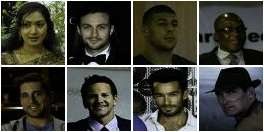
\includegraphics[width=0.3\textwidth]{images/out.png}
\caption{Examples of faces in our dataset.}
\end{figure}

Say we have a 380,639 RGB 64x64 images of the faces of 4,000 different people. We want to identify which person is in each photo. How do we do this? \\

One way to handle this is via a simple classification model. \\

Here's the pipeline:

\begin{enumerate}
    \item We group several images into a batch shaped \ttt{(batch\_size, in\_channels, height, width)}, and pass it into a multi-layer 2d CNN.
    \item The output of this multi-layer 2d CNN is a batch of \textbf{embeddings}, shaped \ttt{(batch\_size, num\_channels, height, width)}. 
    \begin{itemize}
        \item As we've discussed earlier, embeddings are generally abstract representations of the original input images.
        \item But in some cases, embeddings or parts of embeddings can end up representing easily interpretable information, like explicit representations of things like the distance between ears, the relative positioning and size of the eyes, the shape of the head, etc. 
    \end{itemize}
    \item We average these embeddings across the \ttt{height} and \ttt{width} dimensions
\end{enumerate}



% One way to handle this is via a simple classification model. Feed in  We feed in each 64x64 image (or more appropriately, batches of images) as an input to a multi-layer CNN, and at the very end of the model, put a \ttt{Linear} layer with \ttt{out\_features=4000}. The final ``

% \begin{figure}[h]
% \centering
% 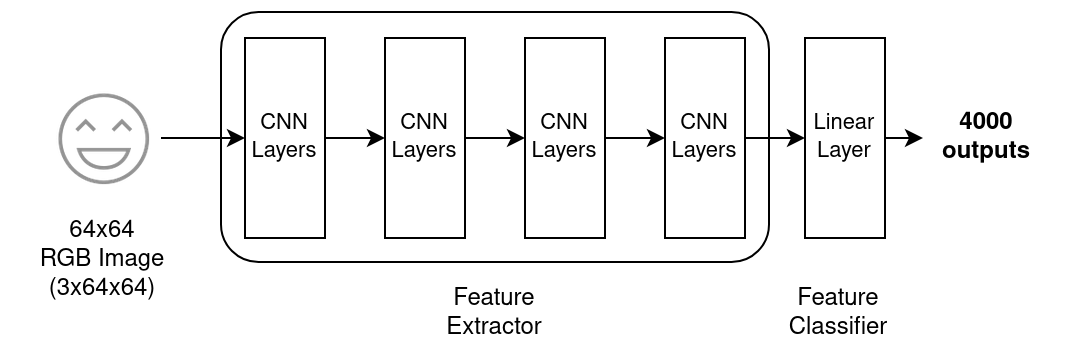
\includegraphics[width=0.8\textwidth]{images/classifier.png}
% \caption{The classification pipeline visualized}
% \end{figure}

% Here's what's going on:

% \begin{itemize}
%     \item The CNN portion of the model is called a \textbf{feature extractor}, as the \textbf{embedding} it creates represents the features of the input image.
%         \begin{itemize}
%             \item The `features' it extracts are often hard to interpret for humans, but in some cases, it can end up explicitly representing details like the distance between ears, the relative positioning and size of the eyes, the shape of the head, etc. 
%         \end{itemize}
%     \item This embedding is then fed to a final linear layer called a \textbf{classifier}, which takes the embedding and determines which of the 4000 classes this face belongs to.
% \end{itemize}

Note that interpreting a model as being an extractor + classifier works for many different types of models in multiple problem spaces. In fact, the phoneme classifier from the first homework can even be interpreted in this way. It's also very common to take the embedding from the second-to-last layer of a trained model and use it for things.

\newpage{}
% --------------------------------------

\section{Verification}
In verification, the goal is to determine whether a given pair of faces belong to the same person. \\

However, \textbf{the people in the verification dataset were NOT in the original classification dataset}. In other words, we want a general model that can verify that two photos are of the same person without assigning specific IDs for that person. \\

Why? Because there are over 7 billion people on earth; classifying across all 7 billion of those people in order to compare them is nearly impossible and unnecessary.\\

This motivates our indirect approach: what if we compared their facial features? \\

Remember that the embeddings from our pretrained classification model encode information about the face in the photo. So if the embeddings are similar enough (i.e. the facial features are similar enough), the faces likely belong to the same person.

% \subsection{The Solution}
% Now let's think about how we might solve this. Recall how the CNN creates a face embedding describing the face, and the linear layer classifies this embedding:

% \begin{figure}[h]
% \centering
% 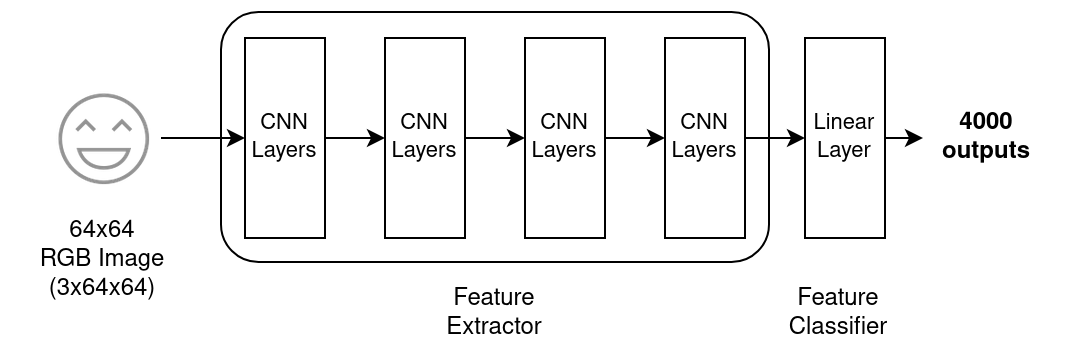
\includegraphics[width=0.4\textwidth]{images/classifier.png}
% \caption{The face classification CNN.}
% \end{figure}

% The hope is that the feature exctractor and thus face embedding is generalizable enough to describe \textbf{any} face, even though the classifier is limited to 4,000 people. If this is the case, than for any two faces, we can calculate the distance between their embeddings, and use the distance to determine if two people are the same:\\

% [image]\\

% Note that just using this scheme will get you okay performance, but you will really want to see the section on center loss to go further.

\subsection{Measuring Similarity}

But how do you precisely measure how `similar' two faces are? \\

Remember that we're working with vector embeddings, which we can interpret as just `points' in some high dimensional space. \\

\textbf{So we could just measure the distance between these two vectors, and apply some kind of threshold to determine if they're similar or not similar.}

\subsection{Euclidean Distance}
\textbf{Note: Don't use this, just explaining.} \\

One way to measure the distance between two points in space is by using \textbf{euclidean distance}.

$$\text{Euclidean}(p,q)=\sqrt{\sum_{i=1}^{n} (q_i - p_i)^2}$$

$$\text{Where $p$ and $q$ are $n$-dimensional vectors.}$$

\textbf{However}, euclidean distance ranges from $[0, \infty]$, so we can't really neatly place a threshold.

\subsubsection{Cosine Similarity}
Instead, we recommend you use \textbf{cosine similarity}, which is neatly bounded between $[0,1]$.

$$\text{CosineSim}(p,q)=\frac{\sum_{i=1}^{n}{p_i}{q_i}}{\sqrt{\sum_{i=1}^n p^{2}_{i}} \sqrt{\sum_{i=1}^n q^{2}_{i}}}$$

(Use \ttt{nn.CosineSimilarity} for this.) \\

After getting your score, you can then apply a threshold of $\geq0.5$ to determine sufficient similarity. \\

Bam, we have an approach for our problem! Now to figure out what model to use.

\newpage
% ------------------

\section{Model: ResNet}

The ResNet model was created in 2015 by \href{https://arxiv.org/abs/1512.03385}{\underline{He, Zhang, Ren, and Sun \ExternalLink}}. \\

It was based on the VGG model ("Visual Geometry Group" at Oxford), developed by \href{https://arxiv.org/abs/1409.1556}{\underline{Simonyan and Zisserman \ExternalLink}} for the ILSVRC 2014 challenge. \\

Its most notable improvement over VGG was the introduction of \textbf{``Residual Connections"} (aka \textbf{``Skip Connections"}) to help facilitate the training of very deep NNs. \\

It was remarkably successful, and has since come to replace VGG as the standard CV model. It's now considered the field's baseline for benchmarking and quick usage. Even in mid-2021, a ResNet variation called MobileNetV3 is allegedly planned to be used for the NeuralHash algorithm in every Apple iPhone (\href{https://www.imore.com/reports-raise-concerns-about-flaw-apple-csam-scanning}{\underline{source \ExternalLink}}).

\subsection{What are Residual/Skip Connections?}
The key to ResNet's success are its \textbf{skip/residual connections}\footnote{Terms are interchangeable, I prefer `skip' as it's more intuitive}. They're so useful, that even in 2021, skip connections now appear in almost every mainstream DL architecture (transformers, YOLOv3, MLP mixer, etc) across many problem spaces. \\

So what are they? \\

Residual/skip connections are simply when you skip a tensor past one or more layers and combine it with the output of some later layer. 

\begin{figure}[h]
\centering
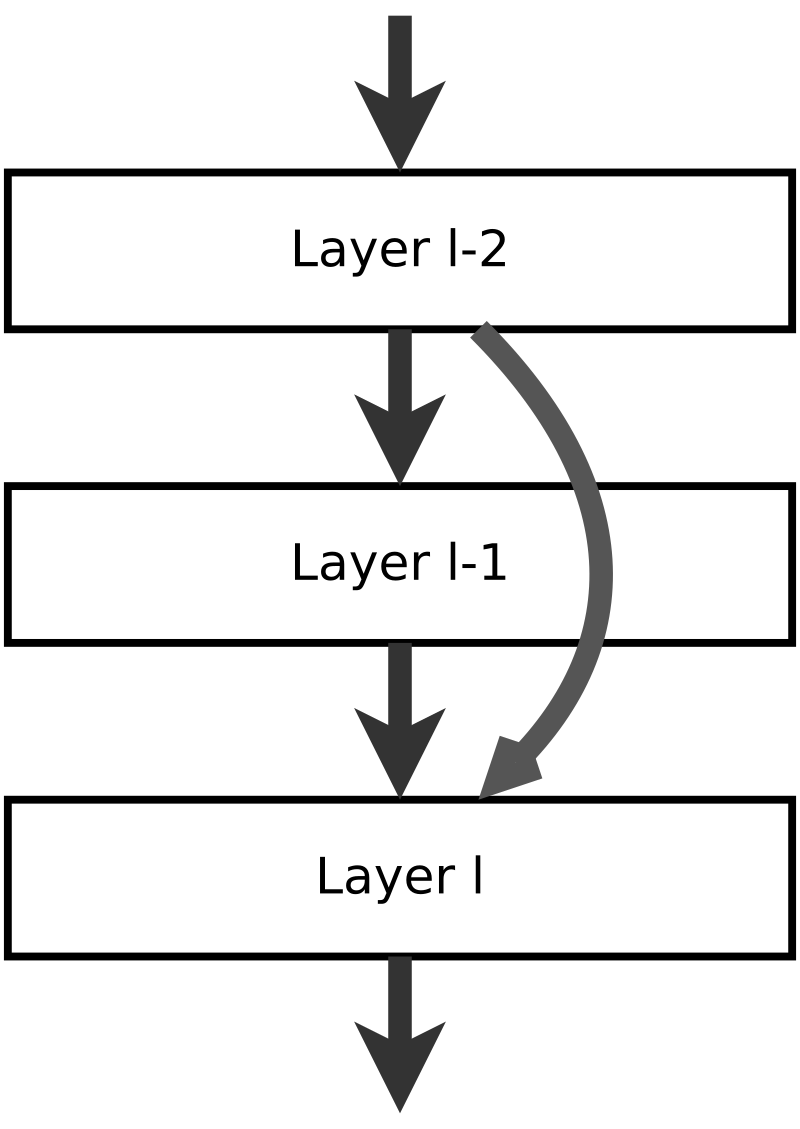
\includegraphics[width=0.3\textwidth]{images/skip_connection.png}
\caption{The output of layer $l-2$ is fed into both $l-1$ AND added to $l-1$'s output. Assume the output of layer $l-2$ and $l-1$ are the same shape for this example.}
\end{figure}

Usually, we add the skipped tensor to a downstream output, but there are variations involving averaging, pooling, etc. \\


\newpage
% --------------------------------------------

\subsection{Why do Skip Connections help?}

While there's no universal consensus on why these work, we do have some generally-accepted hypotheses.  \\

One significant hypothesis is that important information in the original input can be lost or become muddled in later parts of the model. This especially applies for extremely deep models (dozens to hundreds of layers), and also depends on your choice of activation functions. \\

So adding back earlier signals to downstream layers may help preserve the original signals' strength, while still allowing the intermediate layers to extract information. \\

% Empirical studies have also been done on networks with/without skip connections. Those  with them seem to learn faster and smoother, while those without can even fail to converge at all. \\

We won't get into too much detail, but the main takeaways are that skip connections may help preserve signals from earlier in the model, and that they're widely accepted as being helpful in very deep models.

% \newpage
% % -------------------------

\subsection{ResNet Architecture}

The basic unit of ResNet is the ``residual block". These blocks are usually structured identically throughout the model; we just tweak their param sizes and the overall number of blocks there are.  

\begin{figure}[h]
    \centering
    \subfloat[\centering ResBlock with no downsampling]{{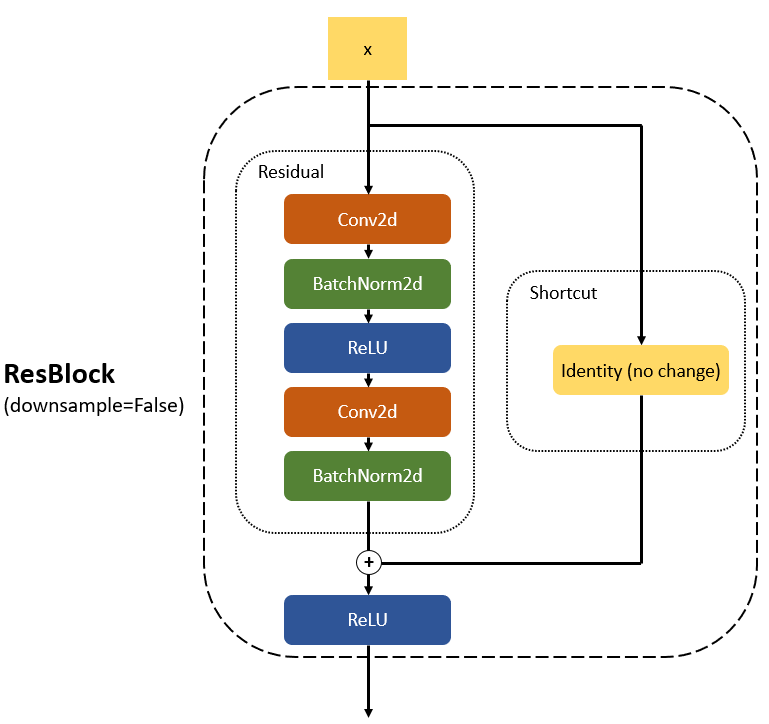
\includegraphics[width=0.5\textwidth]{images/resblock_downsample_false.png}}}%
    % \qquad
    \subfloat[\centering ResBlock with  downsampling]{{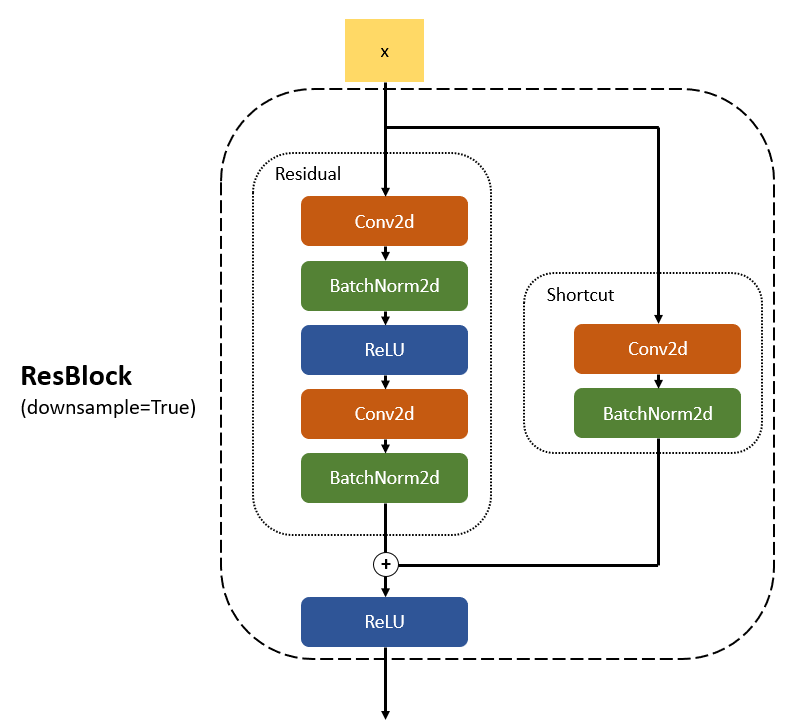
\includegraphics[width=0.5\textwidth]{images/resblock_downsample_true.png}}}%
    \caption{Typical ResBlock, diagram emphasizing how shortcut strategy changes depending on \ttt{downsample} parameter}
\end{figure}

Notice the skip connection from the input of the block to just before the last \ttt{ReLU}. \\

Also note that the architecture changes based on the \ttt{downsample} parameter.

\begin{itemize}
    \item If \ttt{downsample=False}, the first \ttt{Conv2d} in Residual has \ttt{stride=1}, and the shortcut becomes an identity transformation (no change).
    \begin{itemize}
        \item The output will have the same width and height as the input, although the number of channels may have changed.
    \end{itemize}
    \item If \ttt{downsample=True}, the first \ttt{Conv2d} in Residual has \ttt{stride=2}, and the shortcut becomes an additional \ttt{Conv2d}.
\end{itemize}

Don't worry if this seems confusing; we'll walk you through implementing this in the notebook. 

% To see how these parameters change the size of the output tensor, see \href{https://pytorch.org/docs/stable/generated/torch.nn.Conv2d.html}{\underline{this page \ExternalLink}} for some familiar formulas.



% By default,  \\

% However, note that some residual blocks can downsample. This means they double the number of output channels, but half the dimensions of the image. If a block is meant to downsample, then the skip connection will not be the identity; it will have a convolution of stride 2, padding 1, and kernel size 1x1, double the number of output filters as input filters, and a batch normalization after the convolution. In addition, the first convolution in the residual branch will have stride 2, padding 1, and kernel size 3x3, and double the number of output filters. The second residual branch convolution will still have stride 1, padding 1, and kernel size 3x3. \\

% Note that we use padding 1 so that the image size doesn't slowly shrink.

\subsection{Recommended Architecture}

The below table is in order from top to bottom.

\begin{center}
\begin{tabular}{ |c|c|c| } 
 \hline
\ttt{Conv2d(in\_channels=3, out\_channels=64, kernel\_size=3, stride=1, padding=1)}\\
 \hline
\ttt{ResBlock(in\_channels=64, out\_channels=64, kernel\_size=3, downsample=False)}\\
 \hline
\ttt{ResBlock(in\_channels=64, out\_channels=64, kernel\_size=3, downsample=False)}\\
 \hline
\ttt{ResBlock(in\_channels=64, out\_channels=128, kernel\_size=3, downsample=True)}\\
 \hline
\ttt{ResBlock(in\_channels=128, out\_channels=128, kernel\_size=3, downsample=False)}\\
 \hline
\ttt{ResBlock(in\_channels=128, out\_channels=256, kernel\_size=3, downsample=True)}\\
 \hline
\ttt{ResBlock(in\_channels=256, out\_channels=256, kernel\_size=3, downsample=False)}\\
 \hline
\ttt{ResBlock(in\_channels=256, out\_channels=512, kernel\_size=3, downsample=True)}\\
 \hline
\ttt{ResBlock(in\_channels=512, out\_channels=512, kernel\_size=3, downsample=False)}\\
 \hline
Average along last two axes (see section 4.4.1 below)\\
 \hline
\ttt{Linear(512, 4000)}\\
 \hline
\end{tabular}
\end{center}

Notice that \ttt{downsample=True} every time we change the channels. We'll walk you through how to implement downsampling in the notebook.

\subsubsection{Averaging along last axes}

The averaging step is needed to convert our batch of 3D image embeddings into a batch of 1D embeddings.  \\

We need to do this in order to calculate cosine similarity in verification, which is only typically used between 1D vectors. However, we still do this for classification as well, because we try to get the network to make its 1D embeddings as rich as possible.

\begin{verbatim}
Before averaging:
(batch_size, num_channels, height, width)

After averaging:
(batch_size, num_channels)
\end{verbatim}

To do this, you can simply perform \ttt{.mean(dim=2)} twice. \\

\newpage{}
% --------------------------------------


\section{Dataset}

\subsection{Classification Files} 

You'll receive two folders for classification:

\begin{itemize}
    \item \ttt{classification\_train}
        \begin{itemize}
            \item Contains 4,000 subfolders (1 for each person), which contain images of that person's face.
            \item Total: 380,639 RGB images of faces, each sized 64x64
        \end{itemize}
    \item \ttt{classification\_val}
        \begin{itemize}
            \item Same 4,000 people, but only 2 photos per person (8,000 total).
        \end{itemize}
\end{itemize}

These can be very easily loaded in with \ttt{torchvision.datasets.ImageFolder}. Read the documentation for it online to understand how to call and use it. \\

Remember, there is no test data for classification, as you'll only be graded for verification.

\subsection{Verification Files}

You'll receive one folder and two text files for this task.

\begin{itemize}
    \item \ttt{verification\_test}
        \begin{itemize}
            \item No subfolders; contains around 69,000 image files of faces (also RGB and 64x64), each with an integer ID in its filename.
        \end{itemize}
    \item \ttt{verification\_pairs\_test.txt}
        \begin{itemize}
            \item Text file, where each line is space separated (no headers). For example:
    \begin{verbatim}
        verification_data/00041961.jpg verification_data/00044353.jpg 0
    \end{verbatim}
        \item The first two strings are the two images to be compared, and the last integer is a boolean (1 if they're the same person, else 0).
        \end{itemize} 
    \item \ttt{verification\_pairs\_val.txt}
        \begin{itemize}
            \item Same as above. Just in case you want to validate your performance on verification.
        \end{itemize}
\end{itemize}


You can easily load these in with a custom \ttt{Dataset} class we're giving you called \ttt{VerifyDataset}, located in \ttt{utils.py}; make sure you understand how it works.

\newpage{}
% --------------------------------------
\section{Training Tips}

Last section! We'll cover some optimizations for \textbf{speed} of training and inference that we recommend you use to cut down training time.

\subsection*{Introduction: Computer Vision is Expensive!}

A batch of 64 images shaped 64x64 large is represented by $64*64*64*3=786,432$ 32-bit floating point numbers. Each layer performs multiple operations on potentially all of these numbers. \\

And we intentionally gave you smaller images to be kind to your compute needs. A practical CNN may need to process a 1024x512 image. A batch of just 16 of these is $1024\times512\times3\times16=25,165,824$ numbers! \\

In addition, the models themselves are often massive. Their size is well deserved, given that they need to adequately represent the dynamics of objects, shapes, patterns, and their interactions with light in a 3D world. CV models often take gigabytes of memory. And because gradients need to be stored as well, your memory requirement doubles. \\

You get the point; CV is expensive! \\

Below, we'll recommend two techniques you can apply that will reduce the time and memory footprint you'll need to train your model dramatically.

\newpage

\subsection{Technique 1: Automatic Mixed Precision (AMP)}

As stated above, in PyTorch we mostly work with 32-bit \ttt{FloatTensor}s. But for some parts of your pipeline, this level of precision is often unnecessary, and just takes up extra memory and computation. \\

Here's where \textbf{Automatic Mixed Precision (AMP)} comes in.

\subsubsection{What is AMP?}

AMP intelligently detects which parts of your pipeline could use 16-bit precision without hurting performance. It can even find opportunities to re-scale numbers if it'll make scaling to 16-bit precision possible. \\

The benefit of this is so significant that people frequently report between a 30\% to a 300\% speedup to training and inference. When we added it, training time per epoch went from 23 to 13 minutes! \\

For a deeper introduction to AMP, we recommend you read \href{https://docs.nvidia.com/deeplearning/performance/mixed-precision-training/index.html}{\underline{this article by Nvidia \ExternalLink}}.

\subsubsection{\ttt{torch.cuda.amp}}

Thankfully, \ttt{torch} has access to an implementation of this that's reasonably simple to use. \\

We recommend you read \href{https://pytorch.org/docs/stable/notes/amp_examples.html#amp-examples}{\underline{this tutorial \ExternalLink}}. It demonstrates how to use AMP very clearly! \\

The main takeaway is that you'll need to modify your \ttt{train\_epoch()} method in order to get this working. We'll remind you to check the above tutorial at the appropriate part of the notebook.

% . We suggest you read  to learn more, but we will also summarize things here.\\

% Before we use any mixed precision, we generally want to create a gradient scaler. We will cover what this does in a bit.

% \begin{verbatim}
%     gradient_scaler = torch.cuda.amp.GradScaler()
% \end{verbatim}

% In order to calculate things using 16 bits, we use the torch.cuda.ampy.autocast context. This will automatically cast things from 32 bits to 16 bits for us (there are some exceptions, e.g. in-place operations won't get casted). Generally, we calculate only the entire forward pass with auto casting. This is what this might look like:

% \begin{verbatim}
%     with torch.cuda.amp.autocast():
%         out = model(input)
%         total_loss = calc_first_loss(out) + calc_second_loss(out)
% \end{verbatim}


% Next, we perform the backward pass. Gradients that were tiny in 32 bits might now be 0 in 16 bits. To fix that problem, the gradient scaler multiplies the loss by a large number before calling the backward pass:

% \begin{verbatim}
%     gradient_scaler.scale(total_loss).backward()
% \end{verbatim}

% Next, we use the gradient scaler to step the optimizer. Gradient scaling may have creating invalid numbers or infinities, so the grad scaler will intelligently skip the optimizer step if those exist:

% \begin{verbatim}
%     gradient_scaler.step(optimizer)
% \end{verbatim}

% Lastly, the gradient scaler updates its scale internally via the update method:

% \begin{verbatim}
%     gradient_scaler.update()
% \end{verbatim}

% The rest of the training loop is the same! However these ~6 lines of modification can double the speed at which feed forward and convolutional models train, with negligible loss in performance. In our tests, our ResNet goes from 23 minutes an epoch to around 13 with this change.
\newpage{}
% --------------------------------------

\subsection{Technique 2: Center Loss}

\textbf{Center loss} is another loss function you can use in addition to \ttt{CrossEntropyLoss}. And we mean ``in addition" literally, because you add the loss value generated by \ttt{CrossEntropyLoss} to the loss value outputted by \ttt{CenterLoss}. \\

It should help you converge faster, not because it makes the computations faster like AMP did, but because center loss will help your model converge to a better minimum in fewer iterations.

\subsubsection{Motivation: Separating Clusters in Feature Space}

Center loss pushes embeddings of different classes further away from each other. \\

Why is this important? Because our method of measuring similarity between faces relies on a distance metric. So in embedding space, we want faces that are similar to be close to each other, and faces that are different to be farther away. \\

Here's a (very simplified) visualization of center loss's impact on training. \\

\begin{figure}[h]
\centering
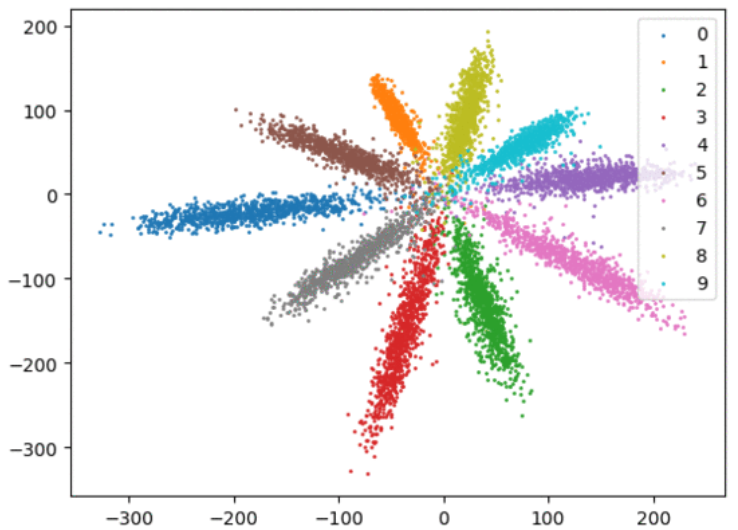
\includegraphics[width=0.4\textwidth]{images/softmax.png}
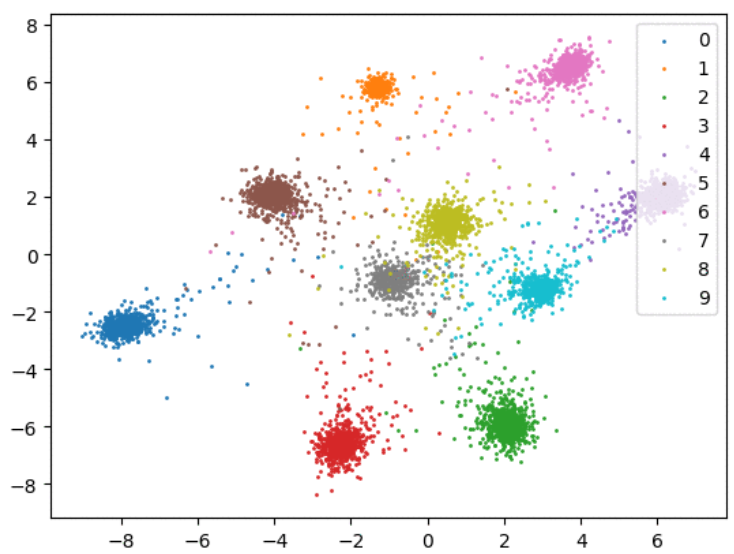
\includegraphics[width=0.4\textwidth]{images/centerloss.png}
\caption{Before and after applying center loss}
\end{figure}

Each point in the plot above represents a single embedding's location in embedding space. Each point is color-coded by class. \\

There are only 10 possible classes in this picture (for us, this would be 4,000 different people). Also notice that the embeddings are just 2-dimensional vectors, instead of the 512-dimensional arrays from our recommended architecture. \\

The main takeaway of the above diagram is that the points close to the middle of the plot are very close together, so it will be hard to differentiate between them using cosine similarity.

\subsubsection{How Center Loss Works}

To address this, center loss coaxes clusters into tighter groups. \\

To do this, it chooses a random center point for each class. It then penalizes embeddings that are far away from those centers. The further away an embedding is from the center point, the more it'll be penalized. 

\subsubsection{How to use it}

We've provided you a full implementation of it that's modified to work with mixed precision. For the code and a detailed readme on how to use it, see \href{https://github.com/KaiyangZhou/pytorch-center-loss}{\underline{here \ExternalLink}}.

\newpage{}
% --------------------------------------


% \subsection{Assignment}

% Now you can start coding! As a recap, here is the order in which you should approach things:

% \begin{itemize}
%     \item Data
%         \begin{itemize}
%             \item Datasets
%             \item Dataloaders
%         \end{itemize}
%     \item Verification
%         \begin{itemize}
%             \item Validate Verification
%             \item Cosine Similarities
%         \end{itemize}
%     \item Train Epoch
%         \item Mixed Precision
%     \item ResNet
%         \begin{itemize}
%             \item ResBlock
%             \item ResNet Architecture
%         \end{itemize}
%     \item Training
%     \item Submission (You should get at least ~0.8)
%     \item CenterLoss (You should get at least ~0.9)
%     \item Further Exploration
% \end{itemize}

\end{document}

% ----------



% As for the architecture, someone might do the following:

% \begin{center}
% \begin{tabular}{ |c|c|c| } 
%  \hline
%  VGGBlock(output filters 32)\\
%   \hline
%  VGGBlock(output filters 64)\\
%   \hline
%  MaxPool(stride 2)\\
%   \hline
%  VGGBlock(output filters 128) x2\\
%   \hline
%  VGGBlock(output filters 256) x2\\
%   \hline
%  MaxPool(stride 2)\\
%   \hline
%  VGGBlock(output filters 256) x2\\
%   \hline
%  MaxPool(stride 2)\\
%   \hline
%  AdaptiveAvgPool2d\\
%   \hline
%  Flatten\\
%   \hline
%  Linear(outputs 4000)\\
%  \hline
% \end{tabular}
% \end{center}


% However... we will not use this model, as it has some in terms of performance. We will instead look at a model from 2015, the residual network (ResNet).